\documentclass[aspectratio=169]{beamer}
% \usepackage{pgfpages}
% \pgfpagesuselayout{4 on 1}[a4paper,landscape,border shrink=5mm]
\usepackage{tikz}
\usetikzlibrary{shapes, backgrounds, arrows, positioning}
%\usepackage{pgfplots}
\usepackage{listings}
\usepackage[utf8,latin1]{inputenc}
\usepackage[style = apa, backend = biber, natbib = true]{biblatex}
\addbibresource{../../literature/lit.bib}

\makeatletter \def\newblock{\beamer@newblock} \makeatother  

\beamertemplatenavigationsymbolsempty
\setbeamertemplate{itemize items}[circle]
\setbeamertemplate{section in toc}[circle]
\mode<beamer>{\setbeamercolor{math text displayed}{fg=iwmgray}}
\setbeamercolor{block body}{bg=iwmorange!50!white}
\setbeamercolor{block title}{fg=white, bg=iwmorange}

% Definitions for biblatex
\setbeamercolor{bibliography entry note}{fg=iwmgray}
\setbeamercolor{bibliography entry author}{fg=iwmgray}
\setbeamertemplate{bibliography item}{}


\definecolor{iwmorange}{RGB}{255,105,0}
\definecolor{iwmgray}{RGB}{67,79,79}
\definecolor{iwmblue}{RGB}{60,180,220}
\definecolor{iwmgreen}{RGB}{145,200,110}
\definecolor{iwmpurple}{RGB}{120,0,75}

\setbeamercolor{title}{fg=iwmorange}
\setbeamercolor{frametitle}{fg=iwmorange}
\setbeamercolor{structure}{fg=iwmorange}
\setbeamercolor{normal text}{fg=iwmgray}
\setbeamercolor{author}{fg=iwmgray}
\setbeamercolor{date}{fg=iwmgray}

\title{Contrast coding in linear (mixed-effects) models}
\author{Nora Wickelmaier}
\date{Last modified: \today}

\newcommand{\vect}[1]{\mathbf{#1}}
\newcommand{\mat}[1]{\mathbf{#1}}
\newcommand{\gvect}[1]{\boldsymbol{#1}}
\newcommand{\gmat}[1]{\boldsymbol{#1}}

\lstset{language = R,%
  basicstyle = \ttfamily\color{iwmgray},
  frame = single,
  rulecolor = \color{iwmgray},
  commentstyle = \slshape\color{iwmgreen},
  keywordstyle = \bfseries\color{iwmgray},
  identifierstyle = \color{iwmpurple},
  stringstyle = \color{iwmblue},
  numbers = none,%left,numberstyle = \tiny,
  basewidth = {.5em, .4em},
  showstringspaces = false,
  emphstyle = \color{red!50!white}}

\pgfmathdeclarefunction{gauss}{2}{%
  \pgfmathparse{1/(#2*sqrt(2*pi))*exp(-((x-#1)^2)/(2*#2^2))}%
}

\AtBeginSection[]{
  \frame{
    \tableofcontents[sectionstyle=show/hide, subsectionstyle=show/show/hide]}}

\setbeamertemplate{headline}{
 \begin{beamercolorbox}{section in head}
   \vskip5pt\insertsectionnavigationhorizontal{\paperwidth}{}{}\vskip2pt
 \end{beamercolorbox}
}

\setbeamertemplate{footline}{\vskip-2pt\hfill\insertframenumber$\;$\vskip2pt}

\begin{document}

\begin{frame}{}
\thispagestyle{empty}
\titlepage
\end{frame}

% \begin{frame}{Outline}
% \tableofcontents
% \end{frame}

\begin{frame}[<+->]{Categorical predictors}
  \begin{itemize}
    \item For all regression models (including mixed-effects model), we need to
      make a choice in how to treat categorical predictors
    \item We need to assign numeric values often called contrasts to our
      categorical variables to enter them into a regression model
    \item Contrasts allow for comparisons between one or more levels of a
      categorical variable
    \item For any categorical variable with $n$ levels, $n - 1$ contrasts (or
      dummy variables) can be defined 
    \item The default contrast in R is the treatment contrast (or dummy coding)
    \item For ANOVAs, so-called sum or effects coding is usually used
  \end{itemize}
\end{frame}

\section[$2\times 2$ example]{$2\times 2$ example for linear mixed-effects model}

\begin{frame}[<+->]{Example by \citet{Brehm2022}}
  \begin{itemize}
    \item We will look at the impact of different contrasts with a small
      simulated example
    \item We have two manipulated factors:
      \begin{enumerate}
        \item \emph{Utensils} with levels \emph{Fork} and \emph{Spoon}
        \item \emph{Foods} with levels \emph{Salad} and \emph{Soup}
      \end{enumerate}
    \item The dependent measure is \emph{RT} (speed of eating in minutes)
    \item We will simulate 20 subjects and 10 food ingredients (items)
    \item The data is generated by the following model
    \only<7>{
      \[
        RT = \beta_0 + \beta_1 Utensils + \beta_2 Foods + \beta_3 Utensils
        \times Foods + \upsilon_0 + \eta_0 + \varepsilon
      \]
    }
    \only<8>{
      \[
        RT = \beta_0 + \beta_1 UtensilsSpoon + \beta_2 FoodsSoup + \beta_3
        UtensilsSpoon \times FoodsSoup + \upsilon_0 + \eta_0 + \varepsilon
      \]
    }
      with $\upsilon_0 \sim N(0, \sigma_{\upsilon}^2)$, $\eta_0 \sim N(0,
      \sigma_{\eta}^2)$, $\varepsilon \sim N(0, \sigma_{\varepsilon}^2)$, all
      i.i.d.
  \end{itemize}
\end{frame}

\begin{frame}[fragile]{Example by \citet{Brehm2022}}
\begin{lstlisting}
library(lme4)
set.seed(1012)

# Average time to eat in min
SpoonSoup  <- 5
ForkSoup   <- 10
SpoonSalad <- 10
ForkSalad  <- 5
# Standard deviation for all groups
Groupsd <- 2
# Number of subjects (ps) and ingredients (ii)
ps <- 20
ii <- 10
\end{lstlisting}
\end{frame}

\begin{frame}[fragile]{Example by \citet{Brehm2022}}
  \small
\begin{lstlisting}
# Create data frame for given design
ds <- data.frame(
  Utensils    = factor(rep(c("Spoon", "Fork"), each = ps * ii, times = 2)),
  Foods       = factor(rep(c("Soup", "Salad"), each = ps * ii * 2)),
  Participant = factor(rep(paste0("p", 1:ps), times = ii * 4)),
  Item        = factor(rep(paste0("i", 1:ii), each = ps, times = 4)))

# Simulate data
ds$RT <- c(rnorm(ps * ii, mean = SpoonSoup,  sd = Groupsd),
           rnorm(ps * ii, mean = ForkSoup,   sd = Groupsd),
           rnorm(ps * ii, mean = SpoonSalad, sd = Groupsd),
           rnorm(ps * ii, mean = ForkSalad,  sd = Groupsd))
psre <- rnorm(ps, mean = 0, sd = Groupsd / 5)
iire <- rnorm(ii, mean = 0, sd = Groupsd / 5)
ds$RT <- ds$RT + psre[ds$Participant] + iire[ds$Item]
\end{lstlisting}
\end{frame}

\begin{frame}[fragile]{Treatment coding}
  \begin{itemize}
    \item The default coding in R is treatment (or dummy) coding
    \item The first level of each factor is assigned as the reference category
\begin{lstlisting}
contrasts(ds$Utensils)
#       Spoon
# Fork      0
# Spoon     1
contrasts(ds$Foods)
#       Soup
# Salad    0
# Soup     1
\end{lstlisting}
  \end{itemize}
\end{frame}

\begin{frame}[fragile]{Effects coding}
  \begin{itemize}
    \item In effects (or sum) coding, one level is set as negative and one
      positive, with zero as the mean of the two levels
    \item For more than two levels, there will also be a reference category,
      which is the \emph{last} factor level in R
\begin{lstlisting}
contrasts(ds$Utensils)
#       [,1]
# Fork     1
# Spoon   -1
contrasts(ds$Foods)
#       [,1]
# Salad    1
# Soup    -1
\end{lstlisting}
  \end{itemize}
\end{frame}

\begin{frame}{}
  \begin{block}{Exercise}
    \begin{itemize}
      \item Fit the model on slide 4 to your simulated data
        \begin{enumerate}
          \item with dummy coding
          \item with effects coding
        \end{enumerate}
      \item Interpret the fixed parameters and compare the variance components
        for the random effects for the two models
      \item What is the interpretation of the intercept for the two models? Why
        does it differ?
    \end{itemize}
  \end{block}
\end{frame}

\begin{frame}{Treatment coding}
  \begin{columns}
    \begin{column}{.45\textwidth}
      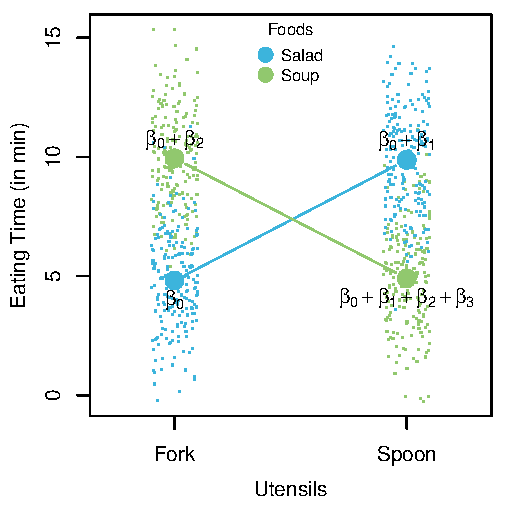
\includegraphics[scale = .8]{../figures/contrasts_dummy}
    \end{column}
    \begin{column}{.5\textwidth}
      \small
      \begin{itemize}
        \item Means from simulated data\vspace{.2cm}
\begin{tabular}{rrr}
  \hline
 & Salad & Soup \\ 
  \hline
Fork & 4.81 & 9.94 \\ 
  Spoon & 9.87 & 4.90 \\ 
   \hline
\end{tabular}
        \item Reference categories: \texttt{Salad} and \texttt{Fork}
        \item Estimated coefficients
      \end{itemize}
      \begin{tabular}{@{}lrrr@{}}
  \hline
 & $\beta$ & SE & $t$ \\ 
  \hline
(Intercept) & 4.81 & 0.21 & 23.45 \\ 
  UtensilsSpoon & 5.06 & 0.20 & 25.19 \\ 
  FoodsSoup & 5.13 & 0.20 & 25.52 \\ 
  UtensilsSpoon:FoodsSoup & -10.10 & 0.28 & -35.52 \\ 
   \hline
\end{tabular}
    \end{column}
  \end{columns}
\end{frame}


\begin{frame}{Effects coding}
  \begin{columns}
    \begin{column}{.45\textwidth}
      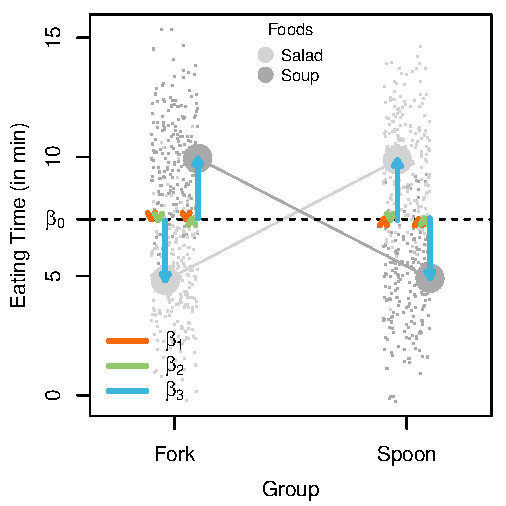
\includegraphics[scale = .8]{../figures/contrasts_effects}
    \end{column}
    \begin{column}{.5\textwidth}
      \small
      \begin{itemize}
        \item Means from simulated data\vspace{.2cm}
\begin{tabular}{rrr}
  \hline
 & Salad & Soup \\ 
  \hline
Fork & 4.81 & 9.94 \\ 
  Spoon & 9.87 & 4.90 \\ 
   \hline
\end{tabular}
        \item Estimated coefficients
      \end{itemize}
      \begin{tabular}{@{}lrrr@{}}
  \hline
 & $\beta$ & SE & $t$ \\ 
  \hline
(Intercept) & 7.38 & 0.16 & 44.97 \\ 
  Utensils1 & -0.01 & 0.07 & -0.09 \\ 
  Foods1 & -0.04 & 0.07 & -0.57 \\ 
  Utensils1:Foods1 & -2.52 & 0.07 & -35.52 \\ 
   \hline
\end{tabular}
    \end{column}
  \end{columns}
\end{frame}

\section{Defining contrasts}

\begin{frame}{General linear model}
  \[
  \vect{y}_i = \mat{X}_i \, \gvect{\beta} + \gvect{\varepsilon}_i
\]
which corresponds to
\[
  \begin{pmatrix}
    y_1 \\
    y_2 \\
    y_3 \\
    \vdots \\
    y_N
  \end{pmatrix} = 
  \begin{pmatrix}
    1 & x_{11} & x_{12} & \dots & x_{1p} \\
    1 & x_{21} & x_{22} & \dots & x_{2p} \\
    1 & x_{31} & x_{32} & \dots & x_{3p} \\
    \vdots & \vdots & \vdots & \vdots & \vdots \\
    1 & x_{N1} & x_{N2} & \dots & x_{Np} \\
  \end{pmatrix} \cdot
  \begin{pmatrix}
    \beta_0 \\
    \beta_1 \\
    \vdots \\
    \beta_p
  \end{pmatrix} +
  \begin{pmatrix}
    \varepsilon_1 \\
    \varepsilon_2 \\
    \varepsilon_3 \\
    \vdots \\
    \varepsilon_N
  \end{pmatrix}
\]
\end{frame}

\begin{frame}[<+->]{Example by \citet{Schad2020}}
  \begin{itemize}
    \item In order to keep it reasonably complex, let us consider a design with
      one between-subjects factor with four levels
    \item The four levels $F_1$ to $F_4$ reflect levels of word frequency with
      levels \texttt{low}, \texttt{medium-low}, \texttt{medium-high}, and
      \texttt{high} frequency words, and the dependent variable reflects some
      response time
    \item From four factor levels, we can build three contrasts
  \end{itemize}
\end{frame}

\begin{frame}{Example by \citet{Schad2020}}
  \begin{columns}
    \begin{column}[t]{.5\textwidth}
  \begin{itemize}
    \item Let us consider 8 subjects for our 4-level between-subjects design
  \end{itemize}
  %\vspace{.2cm}
\[
  \vect{y}_i = \mat{X}_i \, \gvect{\beta} + \gvect{\varepsilon}_i
\]
\[
  \begin{pmatrix}
    y_1 \\
    y_2 \\
    y_3 \\
    y_4 \\
    y_5 \\
    y_6 \\
    y_7 \\
    y_8
  \end{pmatrix} = 
  \begin{pmatrix}
    1 & 0 & 0 & 0 \\ 
    1 & 0 & 0 & 0 \\ 
    1 & 1 & 0 & 0 \\ 
    1 & 1 & 0 & 0 \\ 
    1 & 0 & 1 & 0 \\ 
    1 & 0 & 1 & 0 \\ 
    1 & 0 & 0 & 1 \\ 
    1 & 0 & 0 & 1 \\ 
  \end{pmatrix} \cdot
  \begin{pmatrix}
    \beta_0 \\
    \beta_1 \\
    \beta_2 \\
    \beta_3
  \end{pmatrix} +
  \begin{pmatrix}
    \varepsilon_1 \\
    \varepsilon_2 \\
    \varepsilon_3 \\
    \varepsilon_4 \\
    \varepsilon_5 \\
    \varepsilon_6 \\
    \varepsilon_7 \\
    \varepsilon_8
  \end{pmatrix}
\]
    \end{column}
    \begin{column}[t]{.5\textwidth}
  \begin{itemize}
    \item For the four means of the factor levels, we get
  \end{itemize}
  %\vspace{.2cm}
\[
  \boldsymbol{\mu} = \mat{C} \, \gvect{\beta}
\]
\[
  \begin{pmatrix}
    \mu_1 \\
    \mu_2 \\
    \mu_3 \\
    \mu_4 \\
  \end{pmatrix} = 
  \begin{pmatrix}
    1 & 0 & 0 & 0 \\ 
    1 & 1 & 0 & 0 \\ 
    1 & 0 & 1 & 0 \\ 
    1 & 0 & 0 & 1 \\ 
  \end{pmatrix} \cdot
  \begin{pmatrix}
    \beta_0 \\
    \beta_1 \\
    \beta_2 \\
    \beta_3
  \end{pmatrix}
\]
    \end{column}
  \end{columns}
\end{frame}

\begin{frame}[<+->]{Example by \citet{Schad2020}}
  \begin{itemize}
    \item The contrast matrix $\mat{C}$ defines how the model parameters
      are ``combined'' to estimate $\boldsymbol{\mu}$
    \item $\boldsymbol{\mu}$ is our data and will always be the same
    \item $\mat{C}$ depends on the contrast coding we choose and, therefore, so
      does $\boldsymbol{\beta}$
    \item We will go through different possibilities, all testing different
      hypotheses
      \begin{enumerate}
        \item Treatment contrasts
        \item Sum contrasts
        \item Helmert contrasts
        \item Sequential difference contrasts
        \item Custom contrasts
      \end{enumerate}
  \end{itemize}
\end{frame}

\begin{frame}[fragile]{Example by \citet{Schad2020}}
  \begin{columns}
    \begin{column}{.48\textwidth}
      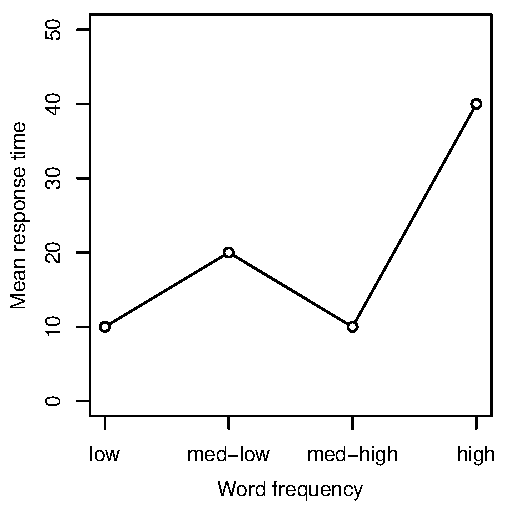
\includegraphics[scale = .8]{../figures/contrasts_ex4level}
    \end{column}
    \begin{column}{.57\textwidth}
\begin{lstlisting}
design <- data.frame(
  F = factor(c("F1", "F2", "F3", "F4")),
  mu = c(10, 20, 10, 40))

beta <- lm(mu ~ F, design) |>
  coef() |>
  zapsmall()
# Contrast matrix
mm <- model.matrix( ~ F, design)

# Compare to mu
mm %*% beta
\end{lstlisting}
    \end{column}
  \end{columns}
\end{frame}

\begin{frame}[<+->]{Contrast vs.\ hypothesis matrix}
  \begin{itemize}
    \item In the literature on contrasts, we sometimes find the distinction
      between contrast and hypothesis matrix \citep[e.\,g.,][]{Schad2020}
    \item When the contrast matrix defines how we add up the parameters to
      obtain $\gvect{\mu}$, then the hypothesis matrix defines how to add up the
      means to obtain the parameters
  \[
    \boldsymbol{\mu} = \mat{C} \, \gvect{\beta} ~~~~~\Leftrightarrow ~~~~~
    \boldsymbol{\beta} = \mat{C}^{-1} \, \gvect{\mu}
  \]
    \item Hence, the hypothesis matrix is the inverse of the contrast matrix
    \item It is sometimes easier to define the hypothesis matrix and then obtain
      the contrast matrix based on it
  \end{itemize}
\end{frame}

\begin{frame}{Treatment contrasts}
  \footnotesize
  Contrast Matrix
  \begin{columns}
    \begin{column}[t]{.5\textwidth}
\[
  \begin{pmatrix}
    \mu_1 \\
    \mu_2 \\
    \mu_3 \\
    \mu_4 \\
  \end{pmatrix} = 
  \begin{pmatrix}
    1 & 0 & 0 & 0 \\ 
    1 & 1 & 0 & 0 \\ 
    1 & 0 & 1 & 0 \\ 
    1 & 0 & 0 & 1 \\ 
  \end{pmatrix} \cdot
  \begin{pmatrix}
    \beta_0 \\
    \beta_1 \\
    \beta_2 \\
    \beta_3
  \end{pmatrix}
\]
    \end{column}
    \begin{column}[t]{.5\textwidth}
\begin{align*}
  \mu_1 & = \beta_0 \\
  \mu_2 & = \beta_0 + \beta_1 \\
  \mu_3 & = \beta_0 + \beta_2 \\
  \mu_4 & = \beta_0 + \beta_3 \\
\end{align*}
    \end{column}
  \end{columns}
  \vspace{-.8cm}
  Hypothesis Matrix
  \begin{columns}
    \begin{column}[t]{.5\textwidth}
\[
  \begin{pmatrix}
    \beta_0 \\
    \beta_1 \\
    \beta_2 \\
    \beta_3 \\
  \end{pmatrix} = 
  \begin{pmatrix}
   1 & 0 & 0 & 0 \\ 
  -1 & 1 & 0 & 0 \\ 
  -1 & 0 & 1 & 0 \\ 
  -1 & 0 & 0 & 1 \\ 
  \end{pmatrix} \cdot
  \begin{pmatrix}
    \mu_1 \\
    \mu_2 \\
    \mu_3 \\
    \mu_4
  \end{pmatrix}
\]
    \end{column}
    \begin{column}[t]{.5\textwidth}
\begin{align*}
  \beta_0 & = \mu_1 \\
  \beta_1 & = \mu_1 - \mu_2 \\
  \beta_2 & = \mu_1 - \mu_3 \\
  \beta_3 & = \mu_1 - \mu_4 \\
\end{align*}
    \end{column}
  \end{columns}
  \vspace{-.8cm}
Hypotheses being tested:
H$_{01}$: $\mu_1 = \mu_2$,
H$_{02}$: $\mu_1 = \mu_3$,
H$_{03}$: $\mu_1 = \mu_4$
\end{frame}

\begin{frame}{Sum contrasts}
  \footnotesize
  Contrast Matrix
  \begin{columns}
    \begin{column}[t]{.5\textwidth}
\[
  \begin{pmatrix}
    \mu_1 \\
    \mu_2 \\
    \mu_3 \\
    \mu_4 \\
  \end{pmatrix} = 
  \begin{pmatrix}
    1 & 1 & 0 & 0 \\ 
    1 & 0 & 1 & 0 \\ 
    1 & 0 & 0 & 1 \\ 
    1 & -1 & -1 & -1 \\ 
  \end{pmatrix} \cdot
  \begin{pmatrix}
    \beta_0 \\
    \beta_1 \\
    \beta_2 \\
    \beta_3
  \end{pmatrix}
\]
    \end{column}
    \begin{column}[t]{.5\textwidth}
\begin{align*}
  \mu_1 & = \beta_0 + \beta_1 \\
  \mu_2 & = \beta_0 + \beta_2 \\
  \mu_3 & = \beta_0 + \beta_3 \\
  \mu_4 & = \beta_0 - \beta_1 - \beta_2 - \beta_3 \\
\end{align*}
    \end{column}
  \end{columns}
  \vspace{-1.2cm}
  Hypothesis Matrix
  \begin{columns}
    \begin{column}[t]{.5\textwidth}
\[
  \begin{pmatrix}
    \beta_0 \\
    \beta_1 \\
    \beta_2 \\
    \beta_3 \\
  \end{pmatrix} = 
  \begin{pmatrix}
     1/4 &  1/4 &  1/4 &  1/4 \\ 
     3/4 & -1/4 & -1/4 & -1/4 \\ 
    -1/4 &  3/4 & -1/4 & -1/4 \\ 
    -1/4 & -1/4 &  3/4 & -1/4 \\ 
  \end{pmatrix} \cdot
  \begin{pmatrix}
    \mu_1 \\
    \mu_2 \\
    \mu_3 \\
    \mu_4
  \end{pmatrix}
\]
    \end{column}
    \begin{column}[t]{.5\textwidth}
\begin{align*}
  \beta_0 & = \frac{\mu_1 + \mu_2 + \mu_3 + \mu_4}{4} \\
  \beta_1 & = \frac{3}{4}\mu_1 - \frac{1}{4}(\mu_2 + \mu_3 + \mu_4)\\
  \beta_2 & = \frac{3}{4}\mu_2 - \frac{1}{4}(\mu_1 + \mu_3 + \mu_4)\\
  \beta_3 & = \frac{3}{4}\mu_3 - \frac{1}{4}(\mu_1 + \mu_2 + \mu_4)\\
\end{align*}
    \end{column}
  \end{columns}
  \vspace{-.8cm}
Hypotheses being tested:
H$_{01}$: $\frac{\mu_2 + \mu_3 + \mu_4}{3} = \mu_1$,
H$_{02}$: $\frac{\mu_1 + \mu_3 + \mu_4}{3} = \mu_2$,
H$_{03}$: $\frac{\mu_1 + \mu_2 + \mu_4}{3} = \mu_3$
\end{frame}

\begin{frame}{Helmert contrasts}
  \footnotesize
  Contrast Matrix
  \begin{columns}
    \begin{column}[t]{.5\textwidth}
\[
  \begin{pmatrix}
    \mu_1 \\
    \mu_2 \\
    \mu_3 \\
    \mu_4 \\
  \end{pmatrix} = 
  \begin{pmatrix}
    1 & -1 & -1 & -1 \\ 
    1 & 1 & -1 & -1 \\ 
    1 & 0 & 2 & -1 \\ 
    1 & 0 & 0 & 3 \\ 
  \end{pmatrix} \cdot
  \begin{pmatrix}
    \beta_0 \\
    \beta_1 \\
    \beta_2 \\
    \beta_3
  \end{pmatrix}
\]
    \end{column}
    \begin{column}[t]{.5\textwidth}
\begin{align*}
  \mu_1 & = \beta_0 - \beta_1 - \beta_2 - \beta_3 \\
  \mu_2 & = \beta_0 + \beta_1 - \beta_2 - \beta_3 \\
  \mu_3 & = \beta_0 +  2\cdot\beta_2 - \beta_3\\
  \mu_4 & = \beta_0 + 3\cdot\beta_3 \\
\end{align*}
    \end{column}
  \end{columns}
  \vspace{-1.2cm}
  Hypothesis Matrix
  \begin{columns}
    \begin{column}[t]{.5\textwidth}
\[
  \begin{pmatrix}
    \beta_0 \\
    \beta_1 \\
    \beta_2 \\
    \beta_3 \\
  \end{pmatrix} = 
  \begin{pmatrix}
   1/4  &  1/4  &  1/4  & 1/4 \\ 
  -1/2  &  1/2  &    0  &   0 \\ 
  -1/6  & -1/6  &  1/3  &   0 \\ 
  -1/12 & -1/12 & -1/12 & 1/4 \\ 
  \end{pmatrix} \cdot
  \begin{pmatrix}
    \mu_1 \\
    \mu_2 \\
    \mu_3 \\
    \mu_4
  \end{pmatrix}
\]
    \end{column}
    \begin{column}[t]{.5\textwidth}
\begin{align*}
  \beta_0 & = \frac{\mu_1 + \mu_2 + \mu_3 + \mu_4}{4} \\
  \beta_1 & = -\frac{1}{2}\mu_1 + \frac{1}{2}\mu_2 \\
  \beta_2 & = -\frac{1}{6}(\mu_1 + \mu_2) + \frac{1}{3}\mu_3 \\
  \beta_3 & = -\frac{1}{12}(\mu_1 + \mu_2 + \mu_3) + \frac{1}{4}\mu_4 \\
\end{align*}
    \end{column}
  \end{columns}
  \vspace{-.8cm}
Hypotheses being tested:
H$_{01}$: $\mu_1 = \mu_2$,
H$_{02}$: $\frac{\mu_1 + \mu_2}{2} = \mu_3$,
H$_{03}$: $\frac{\mu_1 + \mu_2 + \mu_3}{3} = \mu_4$
\end{frame}

\begin{frame}{Sequential difference contrasts}
  \footnotesize
  Contrast Matrix
  \begin{columns}
    \begin{column}[t]{.5\textwidth}
\[
  \begin{pmatrix}
    \mu_1 \\
    \mu_2 \\
    \mu_3 \\
    \mu_4 \\
  \end{pmatrix} = 
  \begin{pmatrix}
  1 & -3/4 & -1/2 & -1/4 \\ 
  1 &  1/4 & -1/2 & -1/4 \\ 
  1 &  1/4 &  1/2 & -1/4 \\ 
  1 &  1/4 &  1/2 &  3/4 \\ 
  \end{pmatrix} \cdot
  \begin{pmatrix}
    \beta_0 \\
    \beta_1 \\
    \beta_2 \\
    \beta_3
  \end{pmatrix}
\]
    \end{column}
    \begin{column}[t]{.5\textwidth}
\begin{align*}
  \mu_1 & = \beta_0 - \frac{3}{4}\beta_1 - \frac{1}{2}\beta_2 - \frac{1}{4}\beta_3 \\
  \mu_2 & = \beta_0 + \frac{1}{4}\beta_1 - \frac{1}{2}\beta_2 - \frac{1}{4}\beta_3 \\
  \mu_3 & = \beta_0 + \frac{1}{4}\beta_1 + \frac{1}{2}\beta_2 - \frac{1}{4}\beta_3 \\
  \mu_4 & = \beta_0 + \frac{1}{4}\beta_1 + \frac{1}{2}\beta_2 + \frac{3}{4}\beta_3 \\
\end{align*}
    \end{column}
  \end{columns}
  \vspace{-1.5cm}
  Hypothesis Matrix
  \begin{columns}
    \begin{column}[t]{.5\textwidth}
\[
  \begin{pmatrix}
    \beta_0 \\
    \beta_1 \\
    \beta_2 \\
    \beta_3 \\
  \end{pmatrix} = 
  \begin{pmatrix}
    1/4 & 1/4 & 1/4 & 1/4 \\ 
     -1 &   1 &   0 &   0 \\ 
      0 &  -1 &   1 &   0 \\ 
      0 &   0 &  -1 &   1 \\ 
  \end{pmatrix} \cdot
  \begin{pmatrix}
    \mu_1 \\
    \mu_2 \\
    \mu_3 \\
    \mu_4
  \end{pmatrix}
\]
    \end{column}
    \begin{column}[t]{.5\textwidth}
\begin{align*}
  \beta_0 & = \frac{\mu_1 + \mu_2 + \mu_3 + \mu_4}{4} \\
  \beta_1 & = \mu_2 - \mu_1 \\
  \beta_2 & = \mu_3 - \mu_2 \\
  \beta_3 & = \mu_4 - \mu_3 \\
\end{align*}
    \end{column}
  \end{columns}
  \vspace{-.8cm}
Hypotheses being tested:
H$_{01}$: $\mu_1 = \mu_2$,
H$_{02}$: $\mu_2 = \mu_3$,
H$_{03}$: $\mu_3 = \mu_4$
\end{frame}

\begin{frame}[<+->]{Custom contrasts}
  \begin{itemize}
    \item All contrasts that we looked at so far are standard and directly
      available in R
    \item It is also possible to construct contrasts testing custom hypotheses
    \item Let us assume for our example, we want to test if the first two
      means ($F_1$ and $F_2$) are identical, but that means for levels $F_3$ and
      $F_4$ increase linearly
    \item Hence, we assume a potential hypothetical outcome, such as $\mu_1 =
      10$, $\mu_2 = 10$, $\mu_3 = 20$, and $\mu_4 = 30$
    \item These means can easily be turned into a contrast by centering them
      and then maybe do some scaling
  \begin{center}
    \begin{tabular}{rrrr}
      \hline
      $\mu_1$ & $\mu_2$ & $\mu_3$ & $\mu_4$ \\
      \hline
      10      & 10      & 20      & 30      \\
      $-$7.5  & $-$7.5  & 2.5     & 12.5    \\
      $-$3    & $-$3    & 1       & 5       \\
      \hline
     \end{tabular}
  \end{center}
  \end{itemize}
\end{frame}

\begin{frame}{Custom contrasts}
  \footnotesize
  Contrast Matrix
  \begin{columns}
    \begin{column}[t]{.5\textwidth}
\[
  \begin{pmatrix}
    \mu_1 \\
    \mu_2 \\
    \mu_3 \\
    \mu_4 \\
  \end{pmatrix} = 
  \begin{pmatrix}
  1 & -3 \\ 
  1 & -3 \\ 
  1 &  1 \\ 
  1 &  5 \\ 
  \end{pmatrix} \cdot
  \begin{pmatrix}
    \beta_0 \\
    \beta_1
  \end{pmatrix}
\]
    \end{column}
    \begin{column}[t]{.5\textwidth}
\begin{align*}
  \mu_1 & = \beta_0 - 3\beta_1 \\
  \mu_2 & = \beta_0 - 3\beta_1 \\
  \mu_3 & = \beta_0 + \beta_1 \\
  \mu_4 & = \beta_0 + 5\beta_1 \\
\end{align*}
    \end{column}
  \end{columns}
  \vspace{-0.8cm}
  Hypothesis Matrix
  \begin{columns}
    \begin{column}[t]{.5\textwidth}
\[
  \begin{pmatrix}
    \beta_0 \\
    \beta_1 \\
  \end{pmatrix} = 
  \begin{pmatrix}
    1/4 & 1/4 & 1/4 & 1/4 \\ 
  -0.068 & -0.068 & 0.023 & 0.114 \\ 
  \end{pmatrix} \cdot
  \begin{pmatrix}
    \mu_1 \\
    \mu_2 \\
    \mu_3 \\
    \mu_4
  \end{pmatrix}
\]
    \end{column}
    \begin{column}[t]{.5\textwidth}
\begin{align*}
  \beta_0 & = \frac{\mu_1 + \mu_2 + \mu_3 + \mu_4}{4} \\
  \beta_1 & = -\frac{3}{44}\mu_1 - \frac{3}{44}\mu_2 + \frac{1}{44}\mu_3 +
  \frac{5}{44}\mu_4 \\
\end{align*}
    \end{column}
  \end{columns}
  %\vspace{-.8cm}
Hypothesis being tested:
H$_{01}$: $-3\mu_1 - 3\mu_2 + \mu_3 + 5\mu_4 = 0$
\end{frame}

\begin{frame}{Custom contrasts}
  \footnotesize
  Contrast Matrix
  \begin{columns}
    \begin{column}[t]{.5\textwidth}
\[
  \begin{pmatrix}
    \mu_1 \\
    \mu_2 \\
    \mu_3 \\
    \mu_4 \\
  \end{pmatrix} = 
  \begin{pmatrix}
  1 & -3 & -0.511 & -0.533 \\ 
  1 & -3 &  0.131 &  0.727 \\ 
  1 &  1 &  0.760 & -0.387 \\ 
  1 &  5 & -0.380 &  0.194 \\ 
  \end{pmatrix} \cdot
  \begin{pmatrix}
    \beta_0 \\
    \beta_1 \\
    \beta_2 \\
    \beta_3
  \end{pmatrix}
\]
    \end{column}
    \begin{column}[t]{.5\textwidth}
      \begin{itemize}
        \item It is often a good idea to add orthogonal contrasts, so any
          variance in your data that is independent of your contrast can be
          accounted for
        \item R will automatically add orthogonal contrasts if you provide less
          than $n - 1$ contrasts for a factor with $n$ levels
      \end{itemize}
    \end{column}
  \end{columns}
  %\vspace{-0.8cm}
  Hypothesis Matrix
  \begin{columns}
    \begin{column}[t]{.5\textwidth}
\[
  \begin{pmatrix}
    \beta_0 \\
    \beta_1 \\
    \beta_2 \\
    \beta_3 \\
  \end{pmatrix} = 
  \begin{pmatrix}
    1/4 & 1/4 & 1/4 & 1/4 \\ 
  -0.068 & -0.068 & 0.023 & 0.114 \\ 
  -0.511 & 0.131 & 0.760 & -0.380 \\ 
  -0.533 & 0.727 & -0.387 & 0.194 \\ 
  \end{pmatrix} \cdot
  \begin{pmatrix}
    \mu_1 \\
    \mu_2 \\
    \mu_3 \\
    \mu_4
  \end{pmatrix}
\]
    \end{column}
    \begin{column}[t]{.5\textwidth}
    \end{column}
  \end{columns}
  \vspace{.1cm}
Hypothesis being tested:
H$_{01}$: $-3\mu_1 - 3\mu_2 + \mu_3 + 5\mu_4 = 0$
\end{frame}

\begin{frame}[fragile]{Simulate data}
\begin{lstlisting}
set.seed(1700)

n <- 20
dat <- data.frame(id = 1:n,
                   F = factor(rep(c("F1", "F2", "F3", "F4"),
                                  times = n / 4)),
                  DV = rnorm(n, mean = c(10, 20, 10, 40), sd = 5)) 

datm <- aggregate(DV ~ F, dat, mean)
aggregate(DV ~ F, dat, sd)

lattice::xyplot(DV ~ F, dat, type = c("a", "p"))
\end{lstlisting}
\end{frame}


\begin{frame}{}
  \begin{block}{Exercise}
    \begin{itemize}
      \item Now fit linear models with all contrasts we looked at
        \begin{enumerate}
          \item Treatment contrasts
          \item Sum contrasts
          \item Helmert contrasts
          \item Sequential difference contrasts
          \item Custom contrasts
        \end{enumerate}
      \item Interpret the fixed parameters
      \item Predict data with each model and compare the results
      \item Look again at the intercepts for all models and compare
    \end{itemize}
  \end{block}
\end{frame}


% TODO:
%
% Look at example by Ben Bolker, maybe use it (or as an exercise?)

\appendix

%\begin{frame}[allowframebreaks]{References}
\begin{frame}{References}
  %\renewcommand{\bibfont}{\footnotesize}
  \printbibliography
  %\vfill
\end{frame}

\end{document}

